\documentclass[
	ngerman,
	toc=listof, % Abbildungsverzeichnis sowie Tabellenverzeichnis in das Inhaltsverzeichnis aufnehmen
	toc=bibliography, % Literaturverzeichnis in das Inhaltsverzeichnis aufnehmen
	footnotes=multiple, % Trennen von direkt aufeinander folgenden Fußnoten
	parskip=half, % vertikalen Abstand zwischen Absätzen verwenden anstatt horizontale Einrückung von Folgeabsätzen
	numbers=noendperiod % Den letzten Punkt nach einer Nummerierung entfernen (nach DIN 5008)
]{scrartcl}
\pdfminorversion=5 % erlaubt das Einfügen von pdf-Dateien bis Version 1.7, ohne eine Fehlermeldung zu werfen (keine Garantie für fehlerfreies Einbetten!)
\usepackage[utf8]{inputenc} % muss als erstes eingebunden werden, da Meta/Packages ggfs. Sonderzeichen enthalten

% !TEX root = Projektdokumentation.tex

% Hinweis: der Titel muss zum Inhalt des Projekts passen und den zentralen Inhalt des Projekts deutlich herausstellen
\newcommand{\titel}{Entwicklung von NatInfo}
\newcommand{\untertitel}{Webbasiertes Tool zur Unterstützung der Entwickler}
\newcommand{\kompletterTitel}{\titel{} -- \untertitel}

\newcommand{\autorName}{Stefan Macke}
\newcommand{\autorAnschrift}{Meine Straße 1}
\newcommand{\autorOrt}{49377 Vechta}

\newcommand{\betriebLogo}{Deloitte.pdf}
\newcommand{\betriebName}{\textsc{Alte Oldenburger} Krankenversicherung AG}
\newcommand{\betriebAnschrift}{Alte-Oldenburger-Platz 1}
\newcommand{\betriebOrt}{49377 Vechta}

\newcommand{\ausbildungsberuf}{Fachinformatiker für Anwendungsentwicklung}
\newcommand{\betreff}{Dokumentation zur betrieblichen Projektarbeit}
\newcommand{\pruefungstermin}{Sommer 2015}
\newcommand{\abgabeOrt}{Vechta}
\newcommand{\abgabeTermin}{23.04.2015}
 % Metadaten zu diesem Dokument (Autor usw.)
% !TEX root = ../Projektdokumentation.tex

% Anpassung an Landessprache ---------------------------------------------------
% \usepackage{babel}
\usepackage[ngerman]{babel}
\usepackage{microtype}

% Umlaute ----------------------------------------------------------------------
%   Umlaute/Sonderzeichen wie äüöß direkt im Quelltext verwenden (CodePage).
%   Erlaubt automatische Trennung von Worten mit Umlauten.
% ------------------------------------------------------------------------------
\usepackage[T1]{fontenc}
\usepackage{textcomp} % Euro-Zeichen etc.

% Schrift ----------------------------------------------------------------------
\usepackage{lmodern} % bessere Fonts
\usepackage{relsize} % Schriftgröße relativ festlegen

% Tabellen ---------------------------------------------------------------------
\PassOptionsToPackage{table}{xcolor}
\usepackage{tabularx}
% für lange Tabellen
\usepackage{longtable}
\usepackage{calc}
\usepackage{array}
\usepackage{ragged2e}
\usepackage{lscape}
\newcolumntype{w}[1]{>{\raggedleft\hspace{0pt}}p{#1}} % Spaltendefinition rechtsbündig mit definierter Breite


% Grafiken ---------------------------------------------------------------------
\usepackage[dvips,final]{graphicx} % Einbinden von JPG-Grafiken ermöglichen
\usepackage{graphics} % keepaspectratio
\usepackage{floatflt} % zum Umfließen von Bildern
\graphicspath{{PA_FISI/}} % hier liegen die Bilder des Dokuments

% Sonstiges --------------------------------------------------------------------
\usepackage[titles]{tocloft} % Inhaltsverzeichnis DIN 5008 gerecht einrücken
% Änderungen am Tabellenverzeichnis vornehmen
% \renewcommand{\cfttabpresnum}{Tabelle }
\renewcommand{\cfttabaftersnum}{\hspace{0.5em}}
% \renewcommand{\cfttabdotsep}{\cftnodots}
\renewcommand{\cfttableader}{\cftdotfill{\cftdotsep}}
\usepackage{amsmath,amsfonts} % Befehle aus AMSTeX für mathematische Symbole
\usepackage{enumitem} % anpassbare Enumerates/Itemizes
\usepackage{xspace} % sorgt dafür, dass Leerzeichen hinter parameterlosen Makros nicht als Makroendezeichen interpretiert werden
\usepackage[utf8]{inputenc}
\usepackage[acronym]{glossaries}
\usepackage{makeidx} % für Index-Ausgabe mit \printindex
\usepackage[printonlyused]{acronym} % es werden nur benutzte Definitionen aufgelistet

% Einfache Definition der Zeilenabstände und Seitenränder etc.
\usepackage{setspace}
\usepackage{geometry}

% Symbolverzeichnis
\usepackage[intoc]{nomencl}
\let\abbrev\nomenclature
\renewcommand{\nomname}{Abkürzungsverzeichnis}
\setlength{\nomlabelwidth}{.25\hsize}
\renewcommand{\nomlabel}[1]{#1 \dotfill}
\setlength{\nomitemsep}{-\parsep}
\usepackage{subcaption}

\usepackage{varioref} % Elegantere Verweise. „auf der nächsten Seite“
\usepackage{url} % URL verlinken, lange URLs umbrechen etc.

\usepackage{chngcntr} % fortlaufendes Durchnummerieren der Fußnoten
% \usepackage[perpage]{footmisc} % Alternative: Nummerierung der Fußnoten auf jeder Seite neu

\usepackage{ifthen} % bei der Definition eigener Befehle benötigt
\usepackage{todonotes} % definiert u.a. die Befehle \todo und \listoftodos
\usepackage[square]{natbib} % wichtig für korrekte Zitierweise

% UML
% \usepackage{tikz}
% \usetikzlibrary{arrows.meta}
% \usepackage{tikz-uml}


% PDF-Optionen -----------------------------------------------------------------
\usepackage{pdfpages}
\pdfminorversion=5 % erlaubt das Einfügen von pdf-Dateien bis Version 1.7, ohne eine Fehlermeldung zu werfen (keine Garantie für fehlerfreies Einbetten!)
\usepackage[
    bookmarks,
    bookmarksnumbered,
    bookmarksopen=true,
    bookmarksopenlevel=1,
    colorlinks=true,
% diese Farbdefinitionen zeichnen Links im PDF farblich aus
    anchorcolor=AOBlau,% Ankertext
    citecolor=AOBlau, % Verweise auf Literaturverzeichniseinträge im Text
    filecolor=AOBlau, % Verknüpfungen, die lokale Dateien öffnen
    menucolor=AOBlau, % Acrobat-Menüpunkte
    urlcolor=AOBlau,
% diese Farbdefinitionen sollten für den Druck verwendet werden (alles schwarz)
    %linkcolor=black, % einfache interne Verknüpfungen
    %anchorcolor=black, % Ankertext
    %citecolor=black, % Verweise auf Literaturverzeichniseinträge im Text
    %filecolor=black, % Verknüpfungen, die lokale Dateien öffnen
    %menucolor=black, % Acrobat-Menüpunkte
    %urlcolor=black,
%
    %backref, % Quellen werden zurück auf ihre Zitate verlinkt
    pdftex,
    plainpages=false, % zur korrekten Erstellung der Bookmarks
    pdfpagelabels=true, % zur korrekten Erstellung der Bookmarks
    hypertexnames=false, % zur korrekten Erstellung der Bookmarks
    linkcolor=black,
    linktoc=all,
]{hyperref}
% Befehle, die Umlaute ausgeben, führen zu Fehlern, wenn sie hyperref als Optionen übergeben werden
\hypersetup{
    pdftitle={\titel -- \untertitel},
    pdfauthor={\autorName},
    pdfcreator={\autorName},
    pdfsubject={\titel -- \untertitel},
    pdfkeywords={\titel -- \untertitel},
}


% zum Einbinden von Programmcode -----------------------------------------------
\usepackage{listings}
\usepackage{xcolor}
\definecolor{hellgelb}{rgb}{1,1,0.9}
\definecolor{colKeys}{rgb}{0,0,1}
\definecolor{colIdentifier}{rgb}{0,0,0}
\definecolor{colComments}{rgb}{0,0.5,0}
\definecolor{colString}{rgb}{1,0,0}
\lstset{
    float=hbp,
	basicstyle=\footnotesize,
    identifierstyle=\color{colIdentifier},
    keywordstyle=\color{colKeys},
    stringstyle=\color{colString},
    commentstyle=\color{colComments},
    backgroundcolor=\color{hellgelb},
    columns=flexible,
    tabsize=2,
    frame=single,
    extendedchars=true,
    showspaces=false,
    showstringspaces=false,
    numbers=left,
    numberstyle=\tiny,
    breaklines=true,
    breakautoindent=true,
	captionpos=b,
}
\lstdefinelanguage{cs}{
	sensitive=false,
	morecomment=[l]{//},
	morecomment=[s]{/*}{*/},
	morestring=[b]",
	morekeywords={
		abstract,event,new,struct,as,explicit,null,switch
		base,extern,object,this,bool,false,operator,throw,
		break,finally,out,true,byte,fixed,override,try,
		case,float,params,typeof,catch,for,private,uint,
		char,foreach,protected,ulong,checked,goto,public,unchecked,
		class,if,readonly,unsafe,const,implicit,ref,ushort,
		continue,in,return,using,decimal,int,sbyte,virtual,
		default,interface,sealed,volatile,delegate,internal,short,void,
		do,is,sizeof,while,double,lock,stackalloc,
		else,long,static,enum,namespace,string},
}
\lstdefinelanguage{natural}{
	sensitive=false,
	morecomment=[l]{/*},
	morestring=[b]",
	morestring=[b]',
	alsodigit={-,*},
	morekeywords={
		DEFINE,DATA,LOCAL,END-DEFINE,WRITE,CALLNAT,PARAMETER,USING,
		IF,NOT,END-IF,ON,*ERROR-NR,ERROR,END-ERROR,ESCAPE,ROUTINE,
		PERFORM,SUBROUTINE,END-SUBROUTINE,CONST,END-FOR,END,FOR,RESIZE,
		ARRAY,TO,BY,VALUE,RESET,COMPRESS,INTO,EQ},
}
\lstdefinelanguage{php}{
	sensitive=false,
	morecomment=[l]{/*},
	morestring=[b]",
	morestring=[b]',
	alsodigit={-,*},
	morekeywords={
		abstract,and,array,as,break,case,catch,cfunction,class,clone,const,
		continue,declare,default,do,else,elseif,enddeclare,endfor,endforeach,
		endif,endswitch,endwhile,extends,final,for,foreach,function,global,
		goto,if,implements,interface,instanceof,namespace,new,old_function,or,
		private,protected,public,static,switch,throw,try,use,var,while,xor
		die,echo,empty,exit,eval,include,include_once,isset,list,require,
		require_once,return,print,unset},
}
 % verwendete Packages
% !TEX root = ../Projektdokumentation.tex

% Seitenränder -----------------------------------------------------------------
\setlength{\topskip}{\ht\strutbox} % behebt Warnung von geometry
\geometry{a4paper,left=20mm,right=20mm,top=25mm,bottom=35mm}

\usepackage[
	automark, % Kapitelangaben in Kopfzeile automatisch erstellen
	headsepline, % Trennlinie unter Kopfzeile
	footsepline, % Trennlinie über Fußzeile
	ilines % Trennlinie linksbündig ausrichten
]{scrlayer-scrpage}

% Kopf- und Fußzeilen ----------------------------------------------------------
\pagestyle{scrheadings}
% chapterpagestyle gibt es nicht in scrartcl
%\renewcommand{\chapterpagestyle}{scrheadings}
\clearscrheadfoot

% Kopfzeile
\renewcommand{\headfont}{\normalfont} % Schriftform der Kopfzeile
\ihead{\large{\textsc{\titel}}\\ \small{\untertitel} \\[2ex] \textit{\headmark}}
\chead{}
% \ohead{\includegraphics[scale=0.1]{\betriebLogo}}
\setlength{\headheight}{20mm} % Höhe der Kopfzeile
\setheadwidth[0mm]{} % Kopfzeile über den Text hinaus verbreitern (falls Logo den Text überdeckt)

% Fußzeile
\ifoot{\autorName}
\setlength{\footheight}{10mm} % Hier die gewünschte Fußzeilenhöhe einstellen
\cfoot{}
\ofoot{\pagemark}

% Überschriften nach DIN 5008 in einer Fluchtlinie
% ------------------------------------------------------------------------------

% Abstand zwischen Nummerierung und Überschrift definieren
% > Schön wäre hier die dynamische Berechnung des Abstandes in Abhängigkeit
% > der Verschachtelungstiefe des Inhaltsverzeichnisses
\newcommand{\headingSpace}{1.5cm}

% Abschnittsüberschriften im selben Stil wie beim Inhaltsverzeichnis einrücken
\renewcommand*{\othersectionlevelsformat}[3]{
  \makebox[\headingSpace][l]{#3\autodot}
}

% Für die Einrückung wird das Paket tocloft benötigt
%\cftsetindents{chapter}{0.0cm}{\headingSpace}
\cftsetindents{section}{0.0cm}{\headingSpace}
\cftsetindents{subsection}{0.0cm}{\headingSpace}
\cftsetindents{subsubsection}{0.0cm}{\headingSpace}
\cftsetindents{figure}{0.0cm}{\headingSpace}
\cftsetindents{table}{0.0cm}{\headingSpace}


% Allgemeines
% ------------------------------------------------------------------------------

\onehalfspacing % Zeilenabstand 1,5 Zeilen
\frenchspacing % erzeugt ein wenig mehr Platz hinter einem Punkt

% Schusterjungen und Hurenkinder vermeiden
\clubpenalty = 10000
\widowpenalty = 10000
\displaywidowpenalty = 10000

% Quellcode-Ausgabe formatieren
\lstset{numbers=left, numberstyle=\tiny, numbersep=5pt, breaklines=true}
\lstset{emph={square}, emphstyle=\color{red}, emph={[2]root,base}, emphstyle={[2]\color{blue}}}

\counterwithout{footnote}{section} % Fußnoten fortlaufend durchnummerieren
\setcounter{tocdepth}{3} % im Inhaltsverzeichnis werden die Kapitel bis zum Level der subsubsection übernommen
\setcounter{secnumdepth}{3} % Kapitel bis zum Level der subsubsection werden nummeriert

% Aufzählungen anpassen
\renewcommand{\labelenumi}{\arabic{enumi}.}
\renewcommand{\labelenumii}{\arabic{enumi}.\arabic{enumii}.}
\renewcommand{\labelenumiii}{\arabic{enumi}.\arabic{enumii}.\arabic{enumiii}}

% Tabellenfärbung:
\definecolor{heading}{rgb}{0.64,0.78,0.86}
\definecolor{odd}{rgb}{0.9,0.9,0.9}
 % Definitionen zum Aussehen der Seiten
% !TEX root = ../Projektdokumentation.tex

% Abkürzungen, ggfs. mit korrektem Leerraum
\newcommand{\bs}{$\backslash$\xspace}
\newcommand{\bspw}{bspw.\xspace}
\newcommand{\bzw}{bzw.\xspace}
\newcommand{\ca}{ca.\xspace}
\newcommand{\dahe}{\mbox{d.\,h.}\xspace}
\newcommand{\etc}{etc.\xspace}
\newcommand{\eur}[1]{\mbox{#1\,\texteuro}\xspace}
\newcommand{\evtl}{evtl.\xspace}
\newcommand{\ggfs}{ggfs.\xspace}
\newcommand{\Ggfs}{Ggfs.\xspace}
\newcommand{\gqq}[1]{\glqq{}#1\grqq{}}
\newcommand{\inkl}{inkl.\xspace}
\newcommand{\insb}{insb.\xspace}
\newcommand{\ua}{\mbox{u.\,a.}\xspace}
\newcommand{\usw}{usw.\xspace}
\newcommand{\Vgl}{Vgl.\xspace}
\newcommand{\zB}{\mbox{z.\,B.}\xspace}

% Befehle für häufig anfallende Aufgaben
\newcommand{\Abbildung}[1]{\autoref{fig:#1}}
\newcommand{\Anhang}[1]{\appendixname{}~\ref{#1}: \nameref{#1} \vpageref{#1}}
\newcommand{\includegraphicsKeepAspectRatio}[2]{\includegraphics[width=#2\textwidth,height=#2\textheight,keepaspectratio]{#1}}
\newcommand{\Zitat}[2][\empty]{\ifthenelse{\equal{#1}{\empty}}{\citep{#2}}{\citep[#1]{#2}}}
\newcommand{\Autor}[1]{\textsc{#1}} % zum Ausgeben von Autoren
\newcommand{\itemd}[2]{\item{\textbf{#1}}\\{#2}} % erzeugt ein Listenelement mit fetter Überschrift

% fügt Tabellen aus einer TEX-Datei ein
\newcommand{\tabelle}[3] % Parameter: caption, label, file
{\begin{table}[htbp]
\centering
\singlespacing
\input{Tabellen/#3}
\caption{#1}
\label{#2}
\end{table}}

\newcommand{\tabelleAnhang}[1] % Parameter: file
{\begin{center}
\singlespacing
\input{Tabellen/#1}
\end{center}}

% einfaches Wechseln der Schrift, z.B.: \changefont{cmss}{sbc}{n}
\newcommand{\changefont}[3]{\fontfamily{#1} \fontseries{#2} \fontshape{#3} \selectfont}

% Verwendung analog zu \includegraphics
\newlength{\myx} % Variable zum Speichern der Bildbreite
\newlength{\myy} % Variable zum Speichern der Bildhöhe
\newcommand\includegraphicstotab[2][\relax]{%
% Abspeichern der Bildabmessungen
\settowidth{\myx}{\includegraphics[{#1}]{#2}}%
\settoheight{\myy}{\includegraphics[{#1}]{#2}}%
% das eigentliche Einfügen
\parbox[c][1.1\myy][c]{\myx}{%
\includegraphics[{#1}]{#2}}%
}

\definecolor{AOBlau}{rgb}{0, 0.28, 0.56}

% verschiedene Befehle um Wörter semantisch auszuzeichnen ----------------------
\newcommand{\Index}[2][\empty]{\ifthenelse{\equal{#1}{\empty}}{\index{#2}#2}{\index{#1}#2}}
\newcommand{\Fachbegriff}[2][\empty]{\ifthenelse{\equal{#1}{\empty}}{\textit{\Index{#2}}}{\textit{\Index[#1]{#2}}}}
\newcommand{\NeuerBegriff}[2][\empty]{\ifthenelse{\equal{#1}{\empty}}{\textbf{\Index{#2}}}{\textbf{\Index[#1]{#2}}}}

\newcommand{\Ausgabe}[1]{\texttt{#1}}
\newcommand{\Eingabe}[1]{\texttt{#1}}
\newcommand{\Code}[1]{\texttt{#1}}
\newcommand{\Datei}[1]{\texttt{#1}}

\newcommand{\Assembly}[1]{\textsf{#1}}
\newcommand{\Klasse}[1]{\textsf{#1}}
\newcommand{\Methode}[1]{\textsf{#1}}
\newcommand{\Attribut}[1]{\textsf{#1}}

\newcommand{\Datentyp}[1]{\textsf{#1}}
\newcommand{\XMLElement}[1]{\textsf{#1}}
\newcommand{\Webservice}[1]{\textsf{#1}}

\newcommand{\Refactoring}[1]{\Fachbegriff{#1}}
\newcommand{\CodeSmell}[1]{\Fachbegriff{#1}}
\newcommand{\Metrik}[1]{\Fachbegriff{#1}}
\newcommand{\DesignPattern}[1]{\Fachbegriff{#1}}
 % eigene allgemeine Befehle, die z.B. die Arbeit mit LaTeX erleichtern
% !TEX root = ../Projektdokumentation.tex

% Abkürzungen, ggfs. mit korrektem Leerraum
\newcommand{\bs}{$\backslash$\xspace}
\newcommand{\bspw}{bspw.\xspace}
\newcommand{\bzw}{bzw.\xspace}
\newcommand{\ca}{ca.\xspace}
\newcommand{\dahe}{\mbox{d.\,h.}\xspace}
\newcommand{\etc}{etc.\xspace}
\newcommand{\eur}[1]{\mbox{#1\,\texteuro}\xspace}
\newcommand{\evtl}{evtl.\xspace}
\newcommand{\ggfs}{ggfs.\xspace}
\newcommand{\Ggfs}{Ggfs.\xspace}
\newcommand{\gqq}[1]{\glqq{}#1\grqq{}}
\newcommand{\inkl}{inkl.\xspace}
\newcommand{\insb}{insb.\xspace}
\newcommand{\ua}{\mbox{u.\,a.}\xspace}
\newcommand{\usw}{usw.\xspace}
\newcommand{\Vgl}{Vgl.\xspace}
\newcommand{\zB}{\mbox{z.\,B.}\xspace}

% Befehle für häufig anfallende Aufgaben
\newcommand{\Abbildung}[1]{\autoref{fig:#1}}
\newcommand{\Anhang}[1]{\appendixname{}~\ref{#1}: \nameref{#1} \vpageref{#1}}
\newcommand{\includegraphicsKeepAspectRatio}[2]{\includegraphics[width=#2\textwidth,height=#2\textheight,keepaspectratio]{#1}}
\newcommand{\Zitat}[2][\empty]{\ifthenelse{\equal{#1}{\empty}}{\citep{#2}}{\citep[#1]{#2}}}
\newcommand{\Autor}[1]{\textsc{#1}} % zum Ausgeben von Autoren
\newcommand{\itemd}[2]{\item{\textbf{#1}}\\{#2}} % erzeugt ein Listenelement mit fetter Überschrift

% fügt Tabellen aus einer TEX-Datei ein
\newcommand{\tabelle}[3] % Parameter: caption, label, file
{\begin{table}[htbp]
\centering
\singlespacing
\input{Tabellen/#3}
\caption{#1}
\label{#2}
\end{table}}

\newcommand{\tabelleAnhang}[1] % Parameter: file
{\begin{center}
\singlespacing
\input{Tabellen/#1}
\end{center}}

% einfaches Wechseln der Schrift, z.B.: \changefont{cmss}{sbc}{n}
\newcommand{\changefont}[3]{\fontfamily{#1} \fontseries{#2} \fontshape{#3} \selectfont}

% Verwendung analog zu \includegraphics
\newlength{\myx} % Variable zum Speichern der Bildbreite
\newlength{\myy} % Variable zum Speichern der Bildhöhe
\newcommand\includegraphicstotab[2][\relax]{%
% Abspeichern der Bildabmessungen
\settowidth{\myx}{\includegraphics[{#1}]{#2}}%
\settoheight{\myy}{\includegraphics[{#1}]{#2}}%
% das eigentliche Einfügen
\parbox[c][1.1\myy][c]{\myx}{%
\includegraphics[{#1}]{#2}}%
}

\definecolor{AOBlau}{rgb}{0, 0.28, 0.56}

% verschiedene Befehle um Wörter semantisch auszuzeichnen ----------------------
\newcommand{\Index}[2][\empty]{\ifthenelse{\equal{#1}{\empty}}{\index{#2}#2}{\index{#1}#2}}
\newcommand{\Fachbegriff}[2][\empty]{\ifthenelse{\equal{#1}{\empty}}{\textit{\Index{#2}}}{\textit{\Index[#1]{#2}}}}
\newcommand{\NeuerBegriff}[2][\empty]{\ifthenelse{\equal{#1}{\empty}}{\textbf{\Index{#2}}}{\textbf{\Index[#1]{#2}}}}

\newcommand{\Ausgabe}[1]{\texttt{#1}}
\newcommand{\Eingabe}[1]{\texttt{#1}}
\newcommand{\Code}[1]{\texttt{#1}}
\newcommand{\Datei}[1]{\texttt{#1}}

\newcommand{\Assembly}[1]{\textsf{#1}}
\newcommand{\Klasse}[1]{\textsf{#1}}
\newcommand{\Methode}[1]{\textsf{#1}}
\newcommand{\Attribut}[1]{\textsf{#1}}

\newcommand{\Datentyp}[1]{\textsf{#1}}
\newcommand{\XMLElement}[1]{\textsf{#1}}
\newcommand{\Webservice}[1]{\textsf{#1}}

\newcommand{\Refactoring}[1]{\Fachbegriff{#1}}
\newcommand{\CodeSmell}[1]{\Fachbegriff{#1}}
\newcommand{\Metrik}[1]{\Fachbegriff{#1}}
\newcommand{\DesignPattern}[1]{\Fachbegriff{#1}}
 % eigene projektspezifische Befehle, z.B. Abkürzungen usw.

\begin{document}

\phantomsection
\thispagestyle{plain}
\pdfbookmark[1]{Deckblatt}{deckblatt}
% !TEX root = Projektdokumentation.tex
\begin{titlepage}

\begin{center}
% 
\includegraphics[scale=0.55]{Bilder/BGB.jpeg}\\[1ex]
\Large{Facharbeit \pruefungstermin}\\[3ex]

% \Large{\ausbildungsberuf}\\
\LARGE{\betreff}\\[10ex]

\huge{\textbf{\titel}}\\[2ex]
\Large{\textbf{\untertitel}}\\[8ex]

\normalsize
Abgabetermin: \abgabeOrt, den \abgabeTermin\\[5em]
\textbf{Schüler:}\\
\autorName\\
\autorAnschrift\\[4em]
% \autorOrt\\[5ex]

\textbf{Betreuer:}\\
\betreuerName\\[6em]

% \includegraphics[scale=0.25]{\betriebLogo}\\[2em]
\textbf{Schule:}\\
\betriebName\\
\betriebAnschrift\\
\betriebOrt\\[5em]
\end{center}

\end{titlepage}
\cleardoublepage


\phantomsection
\thispagestyle{empty}
\pdfbookmark[1]{Projektantrag}{ProjektantragMF}

\includepdf[pages={1-6}]{Anhang/ProjektantragMF.pdf}
\cleardoublepage

% Preface --------------------------------------------------------------------
\phantomsection
\pagenumbering{Roman}
\pdfbookmark[1]{Inhaltsverzeichnis}{inhalt}

% Inhalt ---------------------------------------------------------------------
\pagenumbering{arabic}
% !TEX root = Projektdokumentation.tex

% !TEX root = ../Projektdokumentation.tex
\section{Einleitung}
\label{sec:Einleitung}

\subsection{Projektumfeld} 
\label{sec:Projektumfeld}
Die \cite{Deloitte} Wirtschaftsprüfungsgesellschaft GmbH ist ein internationales 
Unternehmen für Wirtschaftsprüfung, Steuer-, Unternehmens-, Risiko- und Finanzberatung.
Sie hat Niederlassungen in vielen Ländern, darunter auch Deutschland. 
Mit Vertretern in über 150 Ländern weltweit und 415.000 Mitarbeitern, bietet das Unternehmen eine breite Palette 
von Dienstleistungen für Unternehmen und Organisationen in verschiedenen Branchen.
Im \acs{B and TCL}, auch dem Business \& Technology Center Leipzig, erbringt die Deloitte
GmbH mit ihren 100 Mitarbeitern eine Vielfalt an Business Services, mit und ohne IT-Bezug und treibt
Transformationsprojekte rund um die Themen Cyber Security, Digitalisierung,
Prozessoptimierung oder Automatisierung voran. 
\\Das Projekt mit dem Fokus auf Multi-Faktor-Authentifizierung bei verschiedenen Services in einer 
Cloud-Infrastruktur ist ein Tochterprojekt eines Größeren. Dabei ist gemeint, dass dieses 
''Tochterprojekt'' nicht alleine existiert, sondern als Teil des größeren Projektes agiert und es sich 
um ein Subprojekt handelt. Die Deloitte Wirtschaftsprüfungsgesellschaft GmbH verwendet die 
Cloud-Infrastruktur von \cite{ovhcloud}, um einen Business Hosting Service bereitzustellen.
Die Zielgruppe stellt das Projektteam dar, welche in dem größeren Projekt mit entwickeln.

\subsection{Projektaufgabe}
\label{sec:Projektaufgabe}
Der Zweck des Projektes ist es, den Entwicklern der Cloud-Infrastruktur mit den darauf gehosteten Services bzw. 
Diensten, eine Authentifizierungsmöglichkeit zu bieten, die die Sicherheit des Einloggens erhöht.
Die Implementierung der \acs{MFA} steigert nicht nur die Sicherheit, sondern gewährleistet gleichermaßen, 
dass der Zugang zu den Diensten und Daten in der Cloud-Infrastruktur nicht allein durch den Diebstahl eines 
Passworts gefährdet wird. Benutzer müssen zusätzlich zur Eingabe des Nutzernamens und Passwortes einen weiteren 
Authentifizierungsfaktor, wie zum Beispiel ein Einmalkennwort, eingeben. Dabei werden nicht nur firmeninterne und 
kundenbezogene Daten geschützt, sondern auch die Kundenzufriedenheit und das Vertrauen gegenüber der zukünftigen 
Kunden erhöht. Dies hat hohe Priorität und verhindert unbefugten Zugriff auf sensible Informationen.

\subsection{Projektziel} 
\label{sec:Projektziel}
Ziel ist es, die Sicherheit des Zugriffs auf verschiedene Dienste innerhalb dieser Cloud-Infrastruktur zu verbessern, indem 
Multi-Faktor-Authentifizierung (\acs{MFA}) eingeführt wird. Dadurch soll eine erhöhte Sicherheit für firmeninterne und kundenbezogene 
Daten gewährleistet werden, indem nur eine Anmeldung mit \acs{MFA} möglich ist und resultierend daraus Risiken, wie Passwork-Leaks 
und Phishing vermieden werden können.
Um das Ziel zu erreichen, soll eine MFA-Lösung implementiert werden, welche sich vor die verschiedenen Dienste in der 
Cloud-Infrastruktur schaltet und den Zugriff der Benutzer verwalten und sichern soll.

\subsection{Projektschnittstellen} 
\label{sec:Projektschnittstellen}

\subsubsection{Technisch}
\label{sec:Technisch}
Die in Kapitel 1.2 besagte Cloud-Infrastruktur wird in vier  
Hauptbereiche unterteilt, sodass in jedem dieser Bereiche verschiedene Dienste zur Verfügung werden. In jedem dieser Bereiche 
werden die Dienste mittels Docker-Containern initialisiert.
\\\textit{Compliance and Security Stack}
\\Dieser Bereich umfasst den Einsatz, wie die OPNsense Firewall, den NGinx Proxy Manager, dem Authentik- und Guacamole Server 
und Infection Monkey zur Sicherheitsüberprüfung. Zusammenfassend ist zu sagen, dass der NGinx Proxy Manager als Reverse Proxy 
fungiert und den HTTP-Verkehr umleitet und andere Ports für Streaming-Anforderungen bedient. Mittels von Apache Guacamole 
erfolgt die Sicherstellung des Fernzugriffs auf die internen Dienste, die regulär nicht über eine Web-Schnittstelle erreichbar sind.
Das Open-Source-Sicherheitstesttool Infection Monkey überprüft die Sicherheit der Infrastruktur. 
Mit dem Identitätsanbieter \cite{Authentik}, werden verschiedene Identitäts- und Authentifizierungsmethoden in 
Anwendungen und Diensten ermöglicht, zu integrieren. Dadurch wird eine wichtige Schnittstelle für die 
Benutzerauthenfizierung und -autorisierung bereitgestellt und kann von verschiedenen Anwendungen über 
Docker-Container Authentifizierungsmechanismen einrichten.
\\\textit{Monitoring}
\\Im Überwachungsbereich agiert die Open-Source-Software Grafana für die Visualisierung und Überwachung von Leistungsdaten, sowie 
Uptime Kuma als Webserver für Statusseiten und Healtchchecks, um die Verfügbarkeit der Dienste zu kontrollieren. 
\\\textit{DevOps}
\\Der Fokus liegt bei den Anwendungen in der Entwicklung und Bereitstellung und enthält die 
Kollaborationsplattform GitLab, um beispielsweise Projekte zu verwalten. 
Nexus kommt als Verwaltungstool der Repositories für die Anwendungsabhängigkeiten zum Einsatz. Sonarqube ermöglicht die 
statische Analyse und Bewertung der Quelltextqualität. Zusätzlich wird SFTPGo verwendet, um sichere Authentifizierungsmethoden, 
wie zum Beispiele SSH-Schlüssel und Passwörter zu verwalten.
\\\textit{E-Mail-Kommunikation}
\\In diesem Bereich agiert der Mail-Server Mailcow, um E-Mails zu senden und empfangen, SOGO als Groupware-Lösung, 
was eine effiziente E-Mail-Kommunikation und Zusammenarbeit innerhalb und außerhalb des Unternehmens ermöglicht.
\\Für dieses Projekt werden insgesamt drei Instanzen des Anbieters OVHCloud für Cloud-Computing-Dienste genutzt. 
Alle drei Instanzen sind Linux-Systeme mit Ubuntu und variieren in ihren Ressourcen wie RAM und CPU. Auf 
diesen Instanzen werden die im Kapitel genannten Dienste durch Containerisierung gestartet. Jeder Instanz 
wird zur besseren Zuordnung eine spezifische Bezeichnung zugeordnet.
Die erste Instanz, genannt \textbf{''control\_node''}, fungiert als Anlaufstelle, an der sich Benutzer zu Beginn verbinden müssen.
Diese Instanz dient als Kontrollpunkt, über den der Zugang zu den anderen Instanzen erfolgt. Sie fungiert 
gewissermaßen als Gateway zu entweder der Instanz \textbf{''rev\_prox\_dev''} oder der \textbf{''tal\_cloud\_infra''}. 
Der Zugriff auf diese Instanzen geschieht mittels eines \acs{SSH}-Schlüssels von einem lokalen Notebook aus über die Kommandozeile.
Alle Dienste, bis auf den NGinx Reverse Proxy Manager, sind in der ''tal\_cloud\_infra'' lokalisiert. 
Letzterer läuft auf der ''rev\_prox\_dev''-Instanz. Die Bezeichnung ‘‘tal\_cloud\_infra‘‘ bezieht sich auf den Standort Deloitte in Leipzig, bekannt als \acs{TAL}. 
''rev\_prox\_dev'' erhält seinen Namen aufgrund des dort laufenden NGinx Reverse Proxy Managers. Ein Diagramm, das den Zugriff eines Benutzers auf eine Instanz  
über die CLI veranschaulicht, befindet sich im \nameref{sec:Anhang} \nameref{app:Sequenzdiagramm CLI Zugriff auf die Instanzen}.


\subsubsection{Organisatorisch}
\label{sec:Organisatorisch}
Nach der Implementierung der MFA-Lösung in der Cloud-Umgebung, finden erste Tests und Validierungen in den erstellten 
Docker-Containern via der \textit{docker-compose.yml}-Datei statt, um sicherzustellen, dass diese ordnungsgemäß funktioniert und den 
Sicherheitsanforderungen entspricht. 
Im Anschluss erfolgen Schulungen der Benutzer, in dem Fall für das Entwicklerteam, zur genauen Verwendung von Authentik mit \acs{MFA}. 
Nach den Tests und der Schulungen wird die Authentik-\acs{MFA}-Implementierung in der Cloud-Umgebung bereitgestellt.

\subsubsection{Personell}
\label{sec:Personell}
Das Projektteam besteht aus folgenden Personen:
\begin{itemize} [label=--]
	\item Projektleiter/ Manager/ Projektentwickler: Herr Edgar Johann Kapler
	\item Projektentwickler/ dualer Student: Herr Birk Spinn
	\item Projektentwicklerin/ Auszubildende: Frau Melissa Futtig
\end{itemize}
Der Projektleiter ist der Verantwortliche für die Projektleitung und -finanzierung des Projektes. 
Er genehmigt dieses und stellt die notwendigen Ressourcen zur Entwicklung zur Verfügung.
\\Die Projektentwickler sind die allgemeinen Benutzer \bzw das Entwicklerteam. Sie sind für die Umsetzung und den 
reibungslosen Betrieb der Cloud-Infrastruktur verantwortlich und benötigen sichere Zugriffsmöglichkeiten zu den 
bereitgestellten Anwendungen.
% !TEX root = ../Projektdokumentation.tex
\section{Ist/Soll-Analyse} 
\label{sec:IstSollAnalyse}


\subsection{Ist-Analyse} 
\label{sec:IstAnalyse}
Die aktuelle Cloud-Infrastruktur nutzt den NGinx Reverse Proxy Manager für den Zugriff auf verschiedene Dienste. 
Es besteht jedoch keine zusätzliche Sicherheitsschicht wie eine Multi-Faktor-Authentifizierung (\acs{MFA}), 
was bedeutet, dass der Zugriff allein über Benutzernamen- und Passwörtereingabe erfolgt, ohne eine weitere 
Überprüfung der Identität.
% Die Cloud-Umgebung enthält die in den oberen Kapiteln erwähnten Instanzen 
% (\textit{control\_node, rev\_prox\_dev und tal\_cloud\_infra}) und eine OPNSense-Firewall, die den Zugriff 
% von unbefugten Dritten verhindern soll. Die drei Instanzen befinden sich in einem privaten Netzwerk, was 
% bedeutet, dass diesen private nicht von außen sichtbare IP-Adressen zugewiesen werden, während der 
% Firewall eine öffentliche IP-Adresse vergeben wird. 
% Um einen Zugriff auf die Instanzen zu ermöglichen, wird den Command-Line-Interface-Nutzern (\acs{CLI}) mit einem gültigen
% SSH-Schlüssel die Möglichkeit geboten, von der Kontrollinstanz \textit{control\_node} auf die anderen Instanzen 
% zuzugreifen. Die anderen für das Projekt relevanten Instanzen sind \textit{rev\_proxy\_dev} und \textit{tal\_cloud\_infra} 
% auf denen sich, die im Kapitel \ref*{sec:Technisch} \nameref{sec:Technisch}e \nameref{sec:Projektschnittstellen} 
% erwähnten Instanzen befinden. Die Graphical-User-Interface-Nutzer (\acs{GUI}) können die Services über den NGinx Reverse Proxy Manager 
% zu erreichen, indem der Zugriff klassisch mittels einer einfachen Nutzer- und Passworteingabe, ohne einer weiteren 
% Schutzebene erfolgt.

\subsection{Soll-Analyse}
\label{sec:SollAnalyse}
Das Hauptziel besteht darin, die Sicherheit der Dienste durch die Implementierung einer \acs{MFA}-Lösung 
zu verbessern. Geplant ist, vor jedem Dienst einen Identitätsanbieter zu schalten, um sicherzustellen, 
dass sich die \acs{MFA} vor den Diensten positioniert. Benutzer sollen sich über die \acs{MFA} 
authentifizieren, um den Identitätsbestätigungsprozess zu erfüllen und Zugang zu den Diensten zu 
erhalten.


\subsection{Wirtschaftlichkeitsanalyse}
\label{sec:Wirtschaftlichkeitsanalyse}
Durch die schon vorhandene Cloud-Infrastruktur des größeren Projektes entstehen keine weiteren Kosten. Bedingt dessen, dass die 
OVH-Cloud-Infrastruktur zu einem Fix-Preis pro Instanz gemietet wird und keine weiteren Instanzen für die Implementierung 
des Tochter-Projektes erforderlich sind, bleiben die Kosten unverändert. 
An ressourcen wird zwar mehr CPU und Rechenleistung verwendet, was allerdings nicht nach dem \cite{Wiki}-Prinzip 
berechnet wird, sondern bei OVHCloud pauschal nach Instanzpreis, sodass für das ''Tochter-Projekt'' keine weitere 
Kosten entstehen. Die wirklich zu entstehenden Kosten sind ausschließlich Personal- und Materialkosten, wobei letztere 
aus der Nutzung des Büromobiliars und der Strom- und Heizkosten zusammengefasst wird. 
\\Durch die Einführung der \acs{MFA}-Lösung in der Cloud-Infrastruktur werden besonders die Schutzziele der 
Einhaltung der Integrität und Vertraulichkeit der Daten auf den jeweiligen Diensten eingehalten. So wird die Sicherheit 
erheblich verbessert und trägt dazu bei, unbefugten Zugriff, Datenverluste und Betrug zu verhindern. Dieser Schutz 
vor Sicherheitsverletzungen kann erhebliche finanzielle Auswirkungen haben, da die Wiederherstellungskosten vermieden 
werden können. Des Weiteren erfolgen Kostenersparnisse in dem Punkt des Verhinderns der Passwort-Resets durch das Anfragen des 
administrativen Supports, bei welchem Zeit und daraus Kosten entstehen, die vermieden werden können. Durch die Implementierung 
kann den Nutzern ein sicherer und bequemerer Zugriff gewährleistet und die Kosten gesenkt werden.


\subsection{Anforderungsanalyse}
\label{sec:Anforderungsanalyse}

\subsubsection{Funktionale Anforderungen}
\label{sec:Funktional}
Die MFA-Lösung muss folgende funktionale Anforderungen erfüllen:
\begin{itemize} [label=--]
	\item Benutzerfreundliche Registrierung und Login
	\item Klare Anleitung für die Einmalpasswort-Eingabe
	\item Übersichtliche Verwaltung von Nutzern
	\item Einloggen als Admin und Benutzer
	\item Dienste nach Benutzerdateneingabe aktivieren
	\item Schutz vor Drittzugriff, sichere Lösung
	\item Nutzung mit Authentikator-Software
\end{itemize}

\subsubsection{Nicht-Funktionale Anforderungen}
\label{sec:Nicht-Funktional}
Authentik muss folgende nicht-funktionale Anforderungen erfüllen:
\begin{itemize} [label=--]
	\item Skalierbarkeit der Dienste
	\item Übergang zu Diensten in bis zu 2 Sekunden
	\item Übersichtliches Willkommensdisplay (Englisch)
\end{itemize}

% \subsubsection{\gqq{Make or Buy}-Entscheidung}
% \label{sec:MakeOrBuyEntscheidung}
% In der Entscheidungsmatrix für die Zielplattform aus dem Kapitel~\ref{sec:Authentifizierungs-Tool}: \nameref{sec:Authentifizierungs-Tool}
% auf der Seite \pageref{sec:Authentifizierungs-Tool} sind einige alternative Produkte sichtbar, welche wie Authentik, 
% implementiert werden müssen. Daraus resultierend wird sich für Authentik entschieden.

\subsection{Anwendungsfälle}
\label{sec:Anwendungsfaelle}
Ein Use Case-Diagramm zur Veranschaulichung des Prozesses der Cloud-Infrastruktur findet sich im \nameref{sec:Anhang} \ref{app:UseCase} \nameref{app:UseCase}.
In diesem interagiert der Akteur aus der Sicht eines Projektentwicklers mit dem System, in welchem verschiedene 
Anwendungsfälle existieren. Der Akteur meldet sich über den Authentik Server bei der Firewall und dem Nginx Proxy Manager an. 
Nach der erfolgreichen Anmeldung mit der \acs{MFA} hat dieser die Möglichkeit auf die dann zur Verfügung stehenden Dienste vom 
Nginx Reverse Proxy Manager aus zuzugreifen.
\\Hat sich der Akteur mit dem Authentik Server verbunden, der aus dem dem eigentlichen Server (Authentik Server Core) und dem 
integrierten Außenposten (Embedded oupost) besteht, werden einkommende Anfragen an den Server-Containern und den Authentik Server Core 
und dem Embedded oupost geroutet. Der Authentik Core Server verarbeitet den Großteil der Logik von Authentik, wie \zB \acs{API}- und/ oder 
\acs{SSO}-Anfragen, während der Embedded outpost die Verwendung von Proxy-Anbietern ermöglicht, ohne dass eine separate Außenstelle 
eingerichtet werden muss. Der Hintergrundarbeiter (Background Worker) führt Hintergrundaufgaben aus, wie das Senden von E-Mails, 
oder Benachrichtigen von Ereignisses und alles, was im Frontend sichtbar ist. Authentik nutzt PostgreSQL, um alle seiner 
Konfigurationen und Daten zu speichern. Redis wird als Message-Queue und Cache verwendet.
% !TEX root = ../Projektdokumentation.tex
\section{Projektplanung} 
\label{sec:Projektplanung}

\subsection{Projektphasen}
\label{sec:Projektphasen}
Die im Projektantrag festgelegten Projektphasen lassen sich chronologisch in die 8-stündige Planungsphase, 
die 16-stündige Implementierungsphase, die 4-stündige Testphase, die 4-stündige Phase der Einführung und Übergabe 
und die 8-stündige Dokumentation einteilen.
Dabei änderte sich die Zeit in der Implementierungsphase von 14 auf 16 Stunden, die Zeit in der 
Dokumentation von 6 auf 8 Stunden.
\\Das Projekt findet in zwei Wochen, vom 30.10.2023 bis zum 10.11.2023 statt.

Tabelle~\ref{tab:Zeitplanung} \nameref{tab:Zeitplanung} zeigt ein Beispiel für eine grobe Zeitplanung. 
Eine detailliertere Zeitplanung befindet sich im \nameref{sec:Anhang} \nameref{tab:Zeitplanung}.
\tabelle{Zeitplanung}{tab:Zeitplanung}{ZeitplanungKurz}


\subsection{Authentifizierungs-Tool}
\label{sec:Authentifizierungs-Tool}
Anhand der Entscheidungsmatrix in Tabelle~\ref{tab:Nutzwert} wurde Authentik ausgewählt. 
\\Die Gewichtung bildet sich durch den Gesamtwert von 100 Wertungspunkten mit einem Maximalwert von 25 und Mindestwert von 10 Punkten. 
Grund dafür sind die unterschiedlichen Eigenschaften, welche in der Entwicklung und bei der Auswahl der 
Authentifizierungsmethode jeweils verschiedene Rollen spielen und folglich daraus evaluiert werden. Nach der Zuordnung 
und Addierung der Punkte bei den vier Authentifizierungs-Tools, wird die Gesamtheit aller Punkte eines Produktes durch den 
Wert 100 dividiert und das Endergebnis ausgerechnet. Dabei hat die Einhaltung der Sicherheit Priorität und erhält den 
Maximalwert von 25 Punkten, aufgrund dessen, dass Dritten der Zugriff auf die jeweiligen Dienste mit kunden- und 
firmeninternen Daten der Cloud-Infrastruktur verweigert werden sollte. Die \acs{MFA} wird mit 20 Punkten bewertet, weil 
dass das Ziel des Projektes ist. Die Benutzerfreundlichkeit, das Implementieren mit Open-Source und die Skalierbarkeit 
erhalten 15 Punkte, weil jeder User schnell und einfach auf den jeweiligen Dienst zugreifen muss. 
Für dieses Projekt ist es des Weiteren wichtig, ein Tool zu implementieren, was den zeitlichen Rahmen nicht überschreitet und die 
Gesamtheit der Einführung zu komplex gestaltet. Die Skalierbarkeit hat für das Projekt eine durchschnittliche Relevanz, da die 
Möglichkeit bestehen soll, Dienste hinzuzufügen oder rauszunehmen. Am wenigsten bedeutend sind die Erfahrungswerte, welche 
gleichermaßen nicht zu unterschätzen sind, weil eine Community über das Produkt bei der Entwicklung unterstützend wirkend kann.
\\Dabei erhält Authentik den größten Nutzwert mit 17,05 Punkten und schneidet vor Authelia, Microsoft Azure AD und Sitecar am besten ab. 
Aus diesem Grund wird sich für Authentik anstatt für Sitecar entschieden, da besonders die Implementierungsdauer und -komplexität 
bei Sitecar den Rahmen des Projektes sprengen würde.
\tabelle{Entscheidungsmatrix}{tab:Nutzwert}{Nutzwert.tex}
\\Dabei steht \textit{Mic. Az.} für Microsoft Azure.
\\Die zu resultierende Zielplattform definiert sich über die Benutzerfreundlichkeit, die Sicherheit und dem Fokus auf der Interaktion 
mit \acs{OIDC} und \acs{LDAP}, welche zukünftig für das Projekt vorgesehen sind, sowie der Implementierung vom Open-Source, dem Arbeiten mit MFA, 
der Skalierbarkeit und den Erfahrungswerten von anderen Entwicklern mit dem entsprechenden Produkt. Das Resultat wird im Kapitel 
\ref{sec:Authentifizierungs-Tool}: \nameref{sec:Authentifizierungs-Tool} der dargestellten~\nameref{tab:Nutzwert} sichtbar.

\subsection{Ressourcenplanung}
\label{sec:Ressourcenplanung}

\subsubsection{Sachmittelplanung}
\label{sec:Sachmittelplanung}
Um die Umsetzung des Projektes zu ermöglichen, wurden folgende Hard- und Software verwendet:
\begin{itemize} [label=--]
	\item Notebook - Lenovo ThinkPad T15 Gen 1 (für die Entwicklung)
	\item Betriebssystem - Microsoft Windows 10 Enterprise auf dem Lenovo-Notebook
	\item iPhone 12 - iOS 17.0.3 (zum Testen des Einmalpassworts)
	\item Microsoft Authenticator (auf dem iPhone 12 vorinstalliert)
	\item \acs{IDE} - Visual Studio Code 1.83.1 (Benutzereinstellung)
	\item Docker-Containerisierung auf der OVH-Cloud-Infrastruktur in einer Linux-Umgebung mit Ubuntu 22.04
	\item OVH-Cloud-Instanz - firewall\_instance\_dev
	\item OVH-Cloud-Instanz - tal\_cloud\_infra
	\item OVH-Cloud-Instanz - rev\_prox-dev
	\item Google Chrome - Browser
\end{itemize}
Die von OVH-Cloud gestellten Instanzen sind Cloud-Instanzen mit Linux-Umgebungen, auf denen 
die Containerisierungen laufen. Dabei wurde im Kapitel \ref{sec:Projektschnittstellen} 
\nameref{sec:Projektschnittstellen} detaillierter auf die Namen der jeweiligen Instanzen eingegangen.

\subsubsection{Personalplanung}
\label{sec:Personalplanung}
% \paragraph{Tabelle}
Tabelle~\ref{tab:Personalplanung} zeigt die \nameref{tab:Personalplanung} des Projektes.
\tabelle{Personalplanung}{tab:Personalplanung}{Personalplanung.tex}\\
In diesem Projekt arbeitet die Autorin Melissa Futtig 40 Stunden am Projekt, während der Projektmanager 
Edgar Johann Kapler 2 Stunden für das Testen der Anwendung und dem Übergabeprozess aufwendet, da ihm 
das Ergebnis des Projektes schlussendlich übergeben wird. Der duale Student Birk Spinn unterstützt bei 
der Implementierung und dem Testen der Anwendung und benötigt für diese Aufgaben insgesamt 3 Stunden.

\subsection{Kostenplanung}
\label{sec:Kostenplanung}
Die Kosten für die Durchführung des Projekts setzen sich aus den Personal- und Ressourcenkosten zusammen.   
Das Brutto-Einkommen eines Auszubildenden im 3. Lehrjahr im Fachbereich Fachinformatik bei der Deloitte Wirtschaftsprüfungsgesellschaft GmbH 
beträgt \eur{1400,00} pro Monat. Zu den \eur{1400,00} kommen \eur{1090,00} Versicherungskosten dazu, die die Deloitte bezahlt. 
Die reguläre Arbeitszeit in einer normalen Arbeitswoche von Montag bis Freitag beträgt 40 Stunden, 8 Stunden am Tag und 
220 Arbeitstage im Jahr. Die 220 Tage entstehen, da von den 365 Tagen eines Kalenderjahres 104 Wochenendtage, 11 Feiertage und 30 Urlaubstage abgezogen.
Für die weiteren Mitarbeiter werden pauschale Beträge zur Berechnung des Stundensatzes genutzt. 
Duale Studenten werden pauschal mit \eur{15,00}, während die Manager mit \eur{75,00} pro Stunde berechnet werden. 
Bei jeweils beiden addiert sich die Summe der Ressourcenkosten auf.
Anhand der oben genannten Formel ergibt sich ein Stundenlohn von \eur{9,55}. Dieser wird aus dem Brutto-Einkommen des Auszubildenden berechnet.
\\Die Durchführungszeit des Projekts beträgt 40 Stunden. 
Die Anforderungen durch die Ressourcen, wie der Stromverbrauch, die zu verwendende Hardware und die Räumlichkeiten, sowie das Büromaterial, 
wie \zB der zu nutzende Monitor, die Peripheriegeräte (Maus, Tastatur, etc.) und das Mobiliar zusammen.
Der Mittelwert wird pauschal mit \eur{15,00} kalkuliert.  
\begin{eqnarray}
	8 \mbox{ h/Tag} \cdot 220 \mbox{ Tage/Jahr} = 1760 \mbox{ h/Jahr}\\
	\eur{2490}\mbox{/Monat} \cdot 12 \mbox{ Monate/Jahr} = \eur{29880} \mbox{/Jahr}\\
	\frac{\eur{29880} \mbox{/Jahr}}{1760 \mbox{ h/Jahr}} \approx \eur{16,98}\mbox{/h}
\end{eqnarray}
\tabelle{Kostenaufstellung}{tab:Kostenaufstellung}{Kostenaufstellung.tex}
Die Gesamtkosten, dargestellt in der Tabelle~\ref{tab:Kostenaufstellung} betragen \eur{1.561,88}.

\subsection{Wirtschaftlichkeitsanalyse}
\label{sec:Wirtschaftlichkeitsanalyse}
Durch die schon vorhandene Cloud-Infrastruktur des größeren Projektes entstehen keine weiteren Kosten. Bedingt dessen, dass die 
OVH-Cloud-Infrastruktur zu einem Fix-Preis pro Instanz gemietet wird und keine weiteren Instanzen für die Implementierung 
des Tochter-Projektes erforderlich sind, bleiben die Kosten unverändert. 
An Ressourcen wird zwar mehr \acs{CPU} und Rechenleistung verwendet, was allerdings nicht nach dem \cite{Wiki}-Prinzip 
berechnet wird, sondern bei OVH-Cloud pauschal nach Instanzpreis, sodass für das ''Tochter-Projekt'' keine weitere 
Kosten entstehen. In dem Pay-As-You-Go-Prinzip werden nur die Ressourcen bezahlt, die auch tatsächlich genutzt werden. 
Die wirklich zu entstehenden Kosten sind ausschließlich Personal- und Materialkosten, wobei letztere 
aus der Nutzung des Büromobiliars und der Strom- und Heizkosten zusammengefasst wird. 
\\Durch die Einführung der \acs{MFA}-Lösung in der Cloud-Infrastruktur werden besonders die Schutzziele der 
Einhaltung der Integrität und Vertraulichkeit der Daten auf den jeweiligen Diensten eingehalten. So wird die Sicherheit 
erheblich verbessert und trägt dazu bei, unbefugten Zugriff, Datenverluste und Betrug zu verhindern. Dieser Schutz 
vor Sicherheitsverletzungen kann erhebliche finanzielle Auswirkungen haben, da die Wiederherstellungskosten vermieden 
werden können. Zusätzlich ermöglicht die Implementierung, dass Passwortänderungen nur auf Anwendungsebene vorgenommen 
werden, wodurch weniger Zurücksetzungen erforderlich sind. Dies reduziert die Wahrscheinlichkeit von gleichen Passwörtern 
und verhindert dadurch den Bedarf an administrativem Support für Passwort-Resets, wodurch Zeit- und Kostenaufwände vermieden 
werden können. Durch die Implementierung kann den Nutzern ein sicherer und bequemerer Zugriff gewährleistet und die Kosten gesenkt werden. 
Die Einsicht erfolgt in der \nameref{sec:Kostenplanung} im Kapitel \ref{sec:Kostenplanung}.

\subsubsection{Ablaufplanung und Meilensteine}
\label{sec:Ablaufplaung und Meilensteine}
Die Ablaufplanung ist mit einem \nameref{app:Gantt} im Kapitel \ref{app:Gantt} des \nameref{sec:Anhang}s dargestellt. 
Dabei stellt die Farbe pink \textit{keine Arbeitszeit}, die Farbe grün eine \textit{reine Abrbeitszeit} 
von 8 Stunden am Tag und die hellblaue Farbe einen \textit{halben Arbeitstag} von 4 Stunden dar. Die jeweiligen Phasen 
werden mit Meilensteinen abgeschlossen. Die erste Phase startet am Mittwoch, den 01.11.2023, während die letzte 
mit ihrem Meilenstein am 08.11.2023 endet. Dabei erfolgt die reguläre Arbeitszeit in einer normalen Arbeitswoche 
von Montag bis Freitag.

\subsection{Amortisationsdauer}
\label{sec:Amortisationsdauer}
Die Amortisation beschleunigt sich durch die Verwendung von Docker, GitLab und Authentik. 
Grund dafür ist, dass diese Plattformen Open-Source sind und kostenlos genutzt werden können, was zu einer Reduzierung der  
Gesamtbetriebskosten (Total Cost of Ownerships (\acs{TCO})) führt, da Lizenzkosten eingespart werden können.  
% Des Weiteren ermöglicht Docker eine Arbeitszeitersparnis durch die einfache Bereitstellung und Verwaltung von Diensten, was die Arbeitszeit für die 
% Einrichtung und Wartung von Umgebungen verkürzt.
Eine Zeitersparnis entsteht durch das nicht wiederholte Eingeben der Benutzerdaten, zumal sich durch Authentik nur 
einmal eingeloggt werden muss und dadurch ein Zugriff auf alle Applikationen erfolgt.
\\Bei der Einsparung von einer Minute am Tag für jeden der 7 Anwender, nach der dualen Ausbildung und/ oder dem Studium und 
220 Arbeitstagen im Jahr, ergibt sich eine gesamte Zeiteinsparung von 
\begin{eqnarray}
7 \cdot 220 \mbox{ Tage/Jahr} \cdot 1 \mbox{ min/Tag} = 1540 \mbox{ min/Jahr} \approx 25,67 \mbox{ h/Jahr} 
\end{eqnarray}
Die \eur{40} wird der Pauschalbetrag für alle Projektmitarbeiter sein.
\\Die Amortisationszeit setzt sich aus der Division der Gesamtkosten des Projektes und der jährlichen 
Einsparung zusammen.
\\\\$\frac{\eur{1.264,68}}{\eur{1.411,85}\mbox{/Jahr}} \approx 0,90 \mbox{ Jahre} \approx 47 \mbox{ Wochen}$.\\
\\Dadurch ergibt sich eine jährliche Einsparung von 
\begin{eqnarray}
25,67 \mbox{ h} \cdot \eur{(40 + 15)}{\mbox{/h}} = \eur{1.411,85}
\end{eqnarray}

\subsection{Nicht-monetärer Nutzen}
\label{sec:Nicht-monetärer Nutzen}
Für das Projekt werden die Produkte Authelia, Authentik, Microsoft Azure AD und Sitecar, zur Implementierung in Erwägung gezogen. 
Wobei mittels einer Nutzwertanalyse, welche im Kapitel \ref{sec:Authentifizierungs-Tool}: \nameref{sec:Authentifizierungs-Tool} zu sehen ist, der 
Sachverhalt durch eine Entscheidungsmatrix dargestellt wird.
\\Da die Ergebnisse der Wirtschaftlichkeitsanalyse bereits eine ausreichende Begründung für die Umsetzung des Projekts bieten, 
ist es an dieser Stelle nicht notwendig, eine eingehende Untersuchung der nicht-monetären Vorteile vorzunehmen.
\\Ohne der Einführung eines Authentifizierungs-Tools wird die Sicherheit der angebotenen Dienste nicht geboten und das Risiko des 
Datenverlustes gewährleistet. Um das Risiko zu minimieren, soll durch die Nutzwertanalyse ein Ergebnis und die Entscheidungsfindung 
der jeweiligen Authentifizierungsmethode erleichtert werden.

\subsection{Abweichungen vom Projektantrag}
\label{sec:AbweichungenProjektantrag}
Die im Projektantrag mit in \textit{Auflage genehmigt}en Inhalte, erfordern Änderungen in der 
Projektdurchführung und -dokumentation.
\\Erforderliche Änderungen:
\begin{itemize} [label=--]
	\item gesamte Zeitplanung - von 35 auf \textit{40} Stunden gestreckt
	\\Folgen der Zeitänderungen:
	\begin{itemize}
		\item Stundenplanung - Planungsphase von 5 auf \textit{8} Stunden
		\item Stundenplanung - Implementierungsphase von 14 auf \textit{16} Stunden
		\item Stundenplanung - Tesphase von 6 auf \textit{4} Stunden
		\item Stundenplanung - Dokumentation von 8 auf \textit{6} Stunden 
	\end{itemize}
	\item Zeitplanung/ Planungsphase - \textit{Klärung der Projektziele} nach \textit{vorn} der Phase geschoben
	\item Zeitplanung/ Dokumentation - \textit{Benutzerdokumentation} statt Entwicklerdokumentation
\end{itemize}

Nicht erforderliche Änderungen:
\begin{itemize} [label=--]
	\item Implementierungsphase/ Installation und Konfiguration von Sitecars - \textit{Authentik} statt Sitecars
	\\Eine genaue Schilderung, weshalb sich für Authentik anstatt Sitecars entschieden wurde, befindet sich im 
	Kapitel \ref*{sec:Authentifizierungs-Tool} \nameref{sec:Authentifizierungs-Tool}
\end{itemize}

\subsection{Entwicklungsprozess}
\label{sec:Entwicklungsprozess}
Das Projekt unterteilt sich in einem überschaubaren, zeitlich und inhaltlich begrenzten Entwicklungsprozess 
mit gesondert eingeteilten Phasen, die nach- und voneinander aufbauen. So wird eine Sicherstellung der Schritt- 
für Schritt-Fertigstellung der jeweiligen Phasen und Übersicht garantiert. Die klaren und umfassend 
definierten Anforderungen des Projekts ermöglichen eine strukturierte Herangehensweise, die auf 
vorhersehbaren Bedingungen basiert und einen geradlinigen Fortschritt gewährleistet. Auch ist der 
Umfang des Projektes zeitlich eingegrenzt und besitzt eine strukturierte Vorgehensweise mit einer 
geringen Interaktion zum und mit dem Entwicklerteam und des Projektleiters als Kunden.
% !TEX root = ../Projektdokumentation.tex
\section{Entwurfsphase} 
\label{sec:Entwurfsphase}

\subsection{Zielplattform}
\label{sec:Zielplattform}
Die zu resultierende Zielplattform definiert sich über die Benutzerfreundlichkeit, die Sicherheit und dem Fokus auf der Interaktion 
mit \acs{OIDC} und \acs{LDAP}, welche zukünftig für das Projekt vorgesehen sind, sowie der Implementierung vom Open-Source, dem Arbeiten mit MFA, 
der Skalierbarkeit und den Erfahrungswerten von anderen Entwicklern mit dem entsprechenden Produkt. Das Resultat wird im Kapitel 
\ref{sec:Authentifizierungs-Tool}: \nameref{sec:Authentifizierungs-Tool} der dargestellten~\nameref{tab:Nutzwert} sichtbar.


\subsection{Authentifizierungs-Tool}
\label{sec:Authentifizierungs-Tool}
Anhand der Entscheidungsmatrix in Tabelle~\ref{tab:Nutzwert} wurde Authentik ausgewählt. 
\\Die im Kapitel~\ref{sec:Zielplattform}: \nameref{sec:Zielplattform} erwähnten Eigenschaften, tragen zur 
Entscheidungsfindung bei, sodass sich anhand der gegebenen~\nameref{tab:Nutzwert} Authentik herauskristallisierte.
\\Die Gewichtung bildet sich durch den Gesamtwert von 100 Wertungspunkten mit einem Maximalwert von 25 und Mindestwert von 10 Punkten. 
Grund dafür sind die unterschiedlichen Eigenschaften, welche in der Entwicklung und bei der Auswahl der 
Authentifizierungsmethode jeweils verschiedene Rollen spielen und folglich daraus evaluiert werden. Nach der Zuordnung 
und Addierung der Punkte bei den vier Authentifizierungs-Tools, wird die Gesamtheit aller Punkte eines Produktes durch den 
Wert 100 dividiert und das Endergebnis ausgerechnet. Dabei hat die Einhaltung der Sicherheit Priorität und erhält den 
Maximalwert von 25 Punkten, aufgrund dessen, dass Dritten der Zugriff auf die jeweiligen Dienste mit kunden- und 
firmeninternen Daten der Cloud-Infrastruktur verweigert werden sollte. Die \acs{MFA} wird mit 20 Punkten bewertet, weil 
dass das Ziel des Projektes ist. Die Benutzerfreundlichkeit, das Implementieren mit Open-Source und die Skalierbarkeit 
erhalten 15 Punkte, weil jeder User schnell und einfach auf den jeweiligen Dienst zugreifen muss. 
Für dieses Projekt ist es des Weiteren wichtig, ein Tool zu implementieren, was den zeitlichen Rahmen nicht überschreitet und die 
Gesamtheit der Einführung zu komplex gestaltet. Die Skalierbarkeit hat für das Projekt eine durchschnittliche Relevanz, da die 
Möglichkeit bestehen soll, Dienste hinzuzufügen oder rauszunehmen. Am wenigsten bedeutend sind die Erfahrungswerte, welche 
gleichermaßen nicht zu unterschätzen sind, weil eine Community über das Produkt bei der Entwicklung unterstützend wirkend kann.
\\Dabei erhält Authentik den größten Nutzwert mit 17,05 Punkten und schneidet vor Authelia, Microsoft Azure AD und Sitecar am besten ab. 
Aus diesem Grund wird sich für Authentik anstatt für Sitecar entschieden, da besonders die Implementierungsdauer und -komplexität 
bei Sitecar den Rahmen des Projektes sprengen würde.
\tabelle{Entscheidungsmatrix}{tab:Nutzwert}{Nutzwert.tex}

\subsection{Geschäftslogik}
\label{sec:Geschaeftslogik}
Im \nameref{sec:Anhang} befindet sich eine genaue Darstellung der \nameref{app:Cloud-Infrastruktur} und des \nameref{app:UseCase}s, 
sowie das Sequenzdiagramm zur besseren Visualisierung. 
\\Die Implementierung von Authentik erleichert den Entwicklern den Arbeitsfluss durch das einmalige Anmelden bei allen Diensten.

\subsection{Maßnahmen zur Qualitätssicherung}
\label{sec:Qualitaetssicherung}

\subsubsection{Produktorientierte Maßnahmen}
\label{sec:ProduktorientierteMaßnahmen}

\subsubsection{Prozessorientierte Maßnahmen}
\label{sec:ProzessorientierteMaßnahmen}
Durch die kontinuierliche Anwendung des Qualitätsmanagementsystems gemäß ISO 9001 im Qualitätsmanagement erfolgt nach der Planung 
eine sorgfältige Überprüfung jedes Schrittes auf Richtigkeit. Bei festgestellten Fehlern wird nach alternativen Wegen zur 
Zielerreichung gesucht, um diese erfolgreich umzusetzen. Dieser Prozess folgt dem Plan-Do-Check-Act-Zyklus.
\\Als Online-Dienstleister ist es laut den Vorschriften des Bundesamts für Sicherheit in der Informationstechnik (BSI) 
zwingend erforderlich, Daten und Geräte durch eine Mehrfaktor-Authentifizierung (\acs{MFA}) zu schützen, bei der der Login durch 
die Verwendung eines Passworts und eines weiteren Faktors abgesichert wird. Authentik, als Identitätsprovider, nutzt ein 
Informationssicherheitssystem, das auf etablierten Standards wie BSI100-2 und ISO27001 basiert und die Anforderungen erfüllt.
Der Standard BSI 100-2 ist ein Standard des Bundesamtes für Sicherheit in der Informationstechnik, der allgemeine Anforderungen 
an eine Managementsystem für Informationssicherheit (\acs{ISMS}) definiert. Die ISO 27001 ist eine internationale Norm für \acs{ISMS} 
und ist auf der Basis von IT-Grundschutz für die Standard-Absicherung, als auch für die Kern-Absicherung möglich.
% !TEX root = ../Projektdokumentation.tex
\section{Projektdurchführung} 
\label{sec:Projektdurchführung}

\subsection{Vorbereitung der Entwicklungsumgebung}
\label{sec:Vorbereitung der Entwicklungsumgebung}
Die Voraussetzung zur Implementierung von Authentik ist, dass Docker und Docker Compose auf dem im Kapitel \ref{sec:Sachmittelplanung} 
\nameref{sec:Sachmittelplanung} erwähnten Notebook vorinstalliert sind und einen Zugang zum Internet verfügen. Des Weiteren sollten die zu 
benötigenden Hard- und Softwarekomponenten, welche ebenfalls in der \nameref{sec:Sachmittelplanung} auf der Seite \pageref{sec:Sachmittelplanung} 
gelistet sind, funktionierend sein. Wichtig für die Durchführung ist nicht nur Docker mit dem Notebook selbst, sondern auch der 
Besitz einer Domain oder Subdomain, welche bei der Deloitte Wirtschaftsprüfungsgesellschaft GmbH, die \textbf{domain.de} ist. 
Die eigentliche Domain der Deloitte wird mit der \textit{example.domain.de} und später der \textit{auth.example.domain.de} ersetzt.
Diese muss entweder mit einem A- oder CNAME-Record versehen sein. Um die Domain-Names übersichtlich verwalten zu können, 
empfiehlt sich ein Reverse Proxy, in diesem Fall wird es auf den NGinx Proxy Manager zurückzuführen sein. Und zu guter letzt einen SMTP 
E-Mail Server zur beispielsweise Zurücksetzung eines Passworts. Für das Testen der kommenden Schritte im Kapitel 
\ref{sec:Einrichtung des zweiten Faktors} \nameref{sec:Einrichtung des zweiten Faktors} ab der Seite 
\pageref{sec:Einrichtung des zweiten Faktors} wird das iPhone 12, erwähnt in der \nameref{sec:Sachmittelplanung}, verwendet. 
Dieses mobile Endgerät ist ein Firmentelefon und beinhaltet zusätzlich den Microsoft Authenticator, um sich 
gewissermaßen remote mit dem VPN des Firmennetzwerkes verbinden zu können. Aus diesem Grund muss kein weiteres Active Directory 
installiert und eingerichtet werden. Ein Active Directory ist ein Verzeichnisdienst, der gebündelte Informationen zur Verfügung stellt.

\subsection{Auswahl einer MFA-Lösung}
\label{sec:Auswahl einer MFA-Lösung}
Bei Authentik werden die drei Optionen \textbf{WebAuthn Authenticator Setup Stage}, \textbf{Static Authenticator Stage} und 
\textbf{\acs{TOTP} Authenticator Setup Stage} angeboten. 
\\Das Ergebnis der Tabelle \ref*{tab:Nutzwertanalyse} \nameref{tab:Nutzwertanalyse} ist nicht eindeutig zuordbar, bedingt dessen, dass 
die Optionen WebAuthn Authenticator Setup Stage und \acs{TOTP} Authenticator Setup Stage um 0,05 Wertungspunkte auseinander liegen und 
die Entscheidung des finalen Ergebnisses nicht anhand der \nameref{tab:Nutzwertanalyse} manifestierend festzulegen ist.
\tabelle{Nutzwertanalyse zur MFA-Lösung}{tab:Nutzwertanalyse}{Nutzwertanalyse_MFA.tex}
\\Die Entscheidungstreffung erfolgte besonders auf der Prämisse, dass die Deloitte Wirtschaftsprüfungsgesellschaft GmbH das \acs{TOTP}-Verfahren, 
also die Eingabe eines Einmalpassworts, durch einen Authenticator, wie in dem iPhone 12, gestellt durch die Deloitte, bei allen zur Verfügung 
stehenden Diensten verwendet wird. So fiel die Entscheidung auf das \textbf{\acs{TOTP}-Verfahren}, was hingegen zum WebAuth Authenticator 
Setup Stage weniger Sicherheit aber weniger Implementierungsaufwand erfordert und kein weiteres Gerät oder eine weitere Datei oder Software 
notwendig ist, um die in der zu entstehenden hardwarebasierten Token zu verwalten. In dem \acs{TOTP} Authenticator Setup Stage geben die 
Benutzer alle zu Beginn ihren Nutzernamen und das zugehörige Passwort ein. Nach einer erfolgreichen Anmeldung, werden die 
Benutzer weitergeleitet, um ihren 6-stelligen Zahlencode, der in dem Microsoft Authenticator für 30 Sekunden sichtbar ist, einzugeben. 
Wenn die Benutzer sich noch nicht über Authentik angemeldet hatten, werden diese nach der Anmeldung durch einen QR-Code aufgefordert 
den 6-stelligen Code einzugeben.

\subsection{Erstellung der docker-compose.yml, .env}
\label{sec:Erstellung der docker-compose.yml, .env}
Um Authentik über eine \textit{\nameref{app:docker-compose.yml}}-Datei im \nameref{sec:Anhang} des Kapitels \ref{app:docker-compose.yml} 
zum Laufen zu bringen, ist es erforderlich, dass nicht nur der Authenik-Server, sondern auch der Authentik-Worker, 
Redis und PostgreSQL gleichzeitig erstellt werden. PostgreSQL ist eine objektrelationale Datenbank und unterstützt 
die Erweiter- und Skalierbarkeit der Cloud-Infrastruktur. Redis hingegen ist ein In-Memory-Datenspeicher, der als 
schneller Datenspeicher dient. Die ''\nameref{app:dotenv}''-Datei im Kapitel \ref{app:dotenv} \nameref{app:dotenv} 
enthält die individuellen Umgebungsvariablen für die Zugangsdaten der Nutzer :innen. 
\\Beide Dateien werden in einem Ordner ''Authentik'' auf der Instanz \textbf{''tal\_cloud\_infra''} durch docker erstellt. 
Eine Darstellung der Instanzen befindet sich im Kapitel \ref{app:Cloud-Infrastruktur} \nameref{app:Cloud-Infrastruktur}  auf der Seite 
\pageref{app:Cloud-Infrastruktur}. Die ''\nameref{app:docker-compose.yml}''-Datei wurde über \href{https://www.composerize.com/}{Composerize}, einer 
Applikation aus dem Internet entnommen, welche öffentlich zugänglich ist. Auch die ''\nameref{app:dotenv}''-Datei ist öffentlich über die 
Webpage von \href{https://goauthentik.io/}{Authentik} einsehbar. Die einzigen in dieser Datei vorzunehmenden Änderungen, sind die Variablen: 
''PG\_PASS'', ''AUTHENTIK\_SECRET\_KEY'', ''AUTHENTIK\_EMAIL\_\_HOST'', ''AUTHENTIK\_EMAIL\_\_USERNAME'', sowie ''AUTHENTIK\_EMAIL\_\_PASSWORD'' 
und ''AUTHENTIK\_EMAIL\_\_FROM''. Um Authentik zu starten, werden beide Dateien im Unterordner Authentik eingefügt. Nun wird mit dem Befehl 
\textbf{docker-compose pull} in Docker Compose die \textbf{\nameref{app:docker-compose.yml}} mit deren enthaltenen Diensten heruntergeladen, 
die Images und Volumes heruntergezogen. Mit dem Befehl \textbf{docker-compose up -d} erfolgt zu Beginn die Sicherstellung, dass das 
\nameref{app:docker-compose.yml} wirklich vorhanden ist, um dann gelesen und den Container für die darin definierten Dienste im Hintergrund zu starten. Der 
Parameter \textbf{-d (--detach)} bewirkt, dass die Conrainer im Hintergrund ausgeführt werden. Nach dem Start der Container erfolgt die Statusüberprüfung dieser 
mit dem Befehl \textbf{docker-compose ps}. Die Einsicht mit dem Ergebnis der Befehle ist im \nameref{sec:Anhang} \ref{app:dockercommands} 
\nameref{app:dockercommands} einzusehen.

\subsection{Konfiguration des NGinx Reverse Proxy Managers}
\label{sec:Konfiguration des NGinx Reverse Proxy Managers}
Nachdem Authentik in einem Docker-Container läuft, erfolgt die Konfiguration des NGinx Reverse Proxy Managers:
\begin{enumerate}[label=\arabic*.]
    \item Erstellung einer Authentifizierungs-Domain (auth.example.domain) und Einstellung eines A-Records im DNS-Resolver
    \item Im NGinx Reverse Proxy Managers einen neuen Host erstellen, was im \nameref{sec:Anhang} in der \nameref{app:ProxyHostConfig} einsehbar ist
    \item private IP-Adresse des Authentik-Servers mit der in der \textbf{\nameref{app:dotenv}}-Datei eingegebenen Portnummer (80) eingeben 
    mit dem Resultat für das Beispiel: \textbf{0.0.0.0:80} - Einsicht im \ref{app:ProxyHostConfig} \nameref{app:ProxyHostConfig}
    \item im SSL-Tab des Konfigurationsfeldes, anklicken: \textit{Force SSL}, \textit{HTTP/2 Support}, \textit{HSTS Enabled} und \textit{HSTS Subdomains}
    \item im E-Mail Feld die E-Mail Adresse (admin@example.domain.de) eingeben und den Nutzungsbedingungen zustimmen
    \item Ergebnis: Zugriff auf Authentik möglich, sodass die Willkommens-Seite sichtbar wird, welche im \nameref{sec:Anhang} im Kapitel 
    \ref{app:ProxyHostConfig} \nameref{app:ProxyHostConfig}
\end{enumerate}

\subsection{Konfiguration von Authentik}
\label{sec: Konfiguration von Authentik}
Nach der Konfiguration des NGinx Reverse Proxy Managers, werden in Authenik ein Projekt und die vorhandenen User erstellt. Diese Vorgehensweise 
ist im \nameref{sec:Anhang} in der \nameref{app:AuthentikConfig} detailliert beschrieben.
Grobe Vorgehensweise:
\begin{enumerate}
    \item Einrichtung eines Projektes
    \item Erstellung von Benutzern
    \item Hinzufügen des NGinx Proxy Managers
    \item \nameref{sec:Einrichtung des zweiten Faktors} erfolgt in Kapitel \ref*{sec:Einrichtung des zweiten Faktors} auf der 
    Seite \pageref{sec:Einrichtung des zweiten Faktors}
\end{enumerate}


\subsection{Integration mit Cloud-Diensten}
\label{sec:Integration mit Cloud-Diensten}
Damit sich Authentik vor jeden Dienst in der gegebenen Cloud-Infrastruktur schalten kann, wird in der Host-Konfiguration im NGinx Reverse 
Proxy Manager im Bereich \textit{Advanced} die im \nameref{sec:Anhang} erwähnte \nameref{app:CustomNGinxConfig} eingefügt. Wobei zu beachten ist, 
dass bei jedem Dienst die Portnummer geändert werden muss, sodass eine Umleitung von Authelik auf diesen erfolgen kann.

\subsection{Einrichtung des zweiten Faktors}
\label{sec:Einrichtung des zweiten Faktors}
Nach dem Ergebnis aus der \nameref{tab:Nutzwertanalyse} im Kapitel \ref{sec:Auswahl einer MFA-Lösung} \nameref{sec:Auswahl einer MFA-Lösung} 
geht das \acs{TOTP}-Verfahren hervor. Ein Auszug der \nameref{sec:TOTPConfig} im \nameref{sec:Anhang} zeigt die Konfiguration des 
zweiten Faktors.
\\Ein kurze Schrittfolge zur Einrichtung diesens:
\begin{enumerate}
    \item Login bei Authentik
    \item auf \textbf{Einstellungen} gehen und \textbf{\acs{MFA} Devices} bestätigen
    \item \textbf{Enroll} bestätigen - eine Methode auswählen:
    \begin{itemize}
        \item WebAuth Authenticator Setup Stage
        \item Static Authenticator Stage
        \item \textit{TOTP Authenticator Setup Stage} - auswählen
    \end{itemize}
   \item Logout bei Authentik
   \item erneut Login - QR-Code mit Microsoft Azure scannen
   \item 6-stelligen Code eingeben und eingeloggt
\end{enumerate}
% % !TEX root = ../Projektdokumentation.tex
\section{Abnahmephase} 
\label{sec:Abnahmephase}

\begin{itemize} [label=--]
	\item Welche Tests (\zB Unit-, Integrations-, Systemtests) wurden durchgeführt und welche Ergebnisse haben sie geliefert (\zB Logs von Unit Tests, Testprotokolle der Anwender)?
	\item Wurde die Anwendung offiziell abgenommen?
\end{itemize}

\paragraph{Beispiel}
Ein Auszug eines Unit Tests befindet sich im \Anhang{app:Test}. Dort ist auch der Aufruf des Tests auf der Konsole des Webservers zu sehen.

% % !TEX root = ../Projektdokumentation.tex
\section{Einführungsphase}
\label{sec:Einfuehrungsphase}

\begin{itemize}
	\item Welche Schritte waren zum Deployment der Anwendung nötig und wie wurden sie durchgeführt (automatisiert/manuell)?
	\item Wurden \ggfs Altdaten migriert und wenn ja, wie?
	\item Wurden Benutzerschulungen durchgeführt und wenn ja, Wie wurden sie vorbereitet?
\end{itemize}

\section{Testphase}
\label{sec:Testphase}

\subsection{Überwachung der Laufzeit der Services}
\label{Überwachung der Laufzeit der Services}

\subsection{Zugriffstests}
\label{Zugriffstests}
% !TEX root = ../Projektdokumentation.tex
\section{Dokumentation}
\label{sec:Dokumentation}

\begin{itemize} [label=--]
	\item Wie wurde die Anwendung für die Benutzer/Administratoren/Entwickler dokumentiert (\zB Benutzerhandbuch, \acs{API}-Dokumentation)?
	\item Hinweis: Je nach Zielgruppe gelten bestimmte Anforderungen für die Dokumentation (\zB keine IT-Fachbegriffe in einer Anwenderdokumentation verwenden, aber auf jeden Fall in einer Dokumentation für den IT-Bereich).
\end{itemize}

\subsection{Benutzerdokumentation}
\label{sec:Benutzerdokumentation}
Bedingt der internationalen Teams werden bei der Deloitte Wirtschaftsprüfungsgesellschaft GmbH im \acs{B}\&\acs{TCL} Dokumentationen in der 
Sprache Englisch verfasst.

% !TEX root = ../Projektdokumentation.tex
\section{Fazit} 
\label{sec:Fazit}

\subsection{Soll-/Ist-Vergleich}
\label{sec:SollIstVergleich}
Das Projektziel wurde erfolgreich innerhalb des vorgegebenen Zeitrahmens erreicht. Während der Planung stellte sich jedoch heraus, dass die 
geschätzte Dauer der Testphase von ursprünglich 4 Stunden zu grob war und stattdessen in 3 Arbeitsstunden abgeschlossen wurde. Daher wurde die 
übrige 1 Stunde zur Verbesserung der Dokumentation verwendet. Die geplanten Arbeitsstunden für die beiden beteiligten Teammitglieder 
wurden voll ausgeschöpft, und die Ressourcen, wie in der \nameref{sec:Sachmittelplanung} beschrieben, effizient genutzt.
\\Wie in Tabelle~\ref{tab:Vergleich} \nameref{tab:Vergleich} zu erkennen ist, konnte die Zeitplanung bis auf wenige Ausnahmen eingehalten werden.
\tabelle{Soll-/Ist-Vergleich}{tab:Vergleich}{Zeitnachher.tex}

\subsection{Lessons Learned}
\label{sec:LessonsLearned}
Die Zeitplaung und Schätzung der Testphase erwies sich als grob und ungenau. Es ist wichtig zu beachten, realistische Zeitpläne zu erstellen 
und eventuell genügend Puffer einzukalkulieren. Bedingt dessen, dass die Dokumentation ein integraler Bestandteil der Projektarbeit ist, 
wurde die verkürzte Zeit für die Testphase sinnvoll für die Verbesserung der Inhalte in der Dokumetation genutzt. Ein Vorteil der 
ausgewählten \acs{MFA}-Lösung ist, dass die Implementierung recht schnell und nachvollziehbar ging.

\subsection{Ausblick}
\label{sec:Ausblick}
Das Projekt ist eine Tochterprojekt eines übergeordneten Projektes. Mit dem Ergebnis wird die Sicherheit der vorhandenen Dienste gewährleistet. 
Authentik als Identitäts-Provider wird weiter ausgebaut, sodass ein Unternehmensdesign zukünftig erstellt wird und Monitoring-Alerts eingefügt, 
die bei fehlerhaften Logins oder -Logouts eine Mail senden.

% \tableofcontents
% \cleardoublepage

% \phantomsection
% \listoffigures
% \cleardoublepage

\cleardoublepage
\phantomsection
\listoftables
\cleardoublepage

\phantomsection
% \lstlistoflistings
\cleardoublepage

% Literatur ------------------------------------------------------------------
\clearpage
% \renewcommand{\refname}{Literaturverzeichnis}
% \bibliography{Bibliographie}
% \bibliographystyle{Allgemein/natdin} % DIN-Stil des Literaturverzeichnisses
% !TEX root = Projektdokumentation.tex
\clearpage
\addsec{Eidesstattliche Erklärung}

% Hinweis: die eidesstattliche Erklärung ist ggfs. an die Richtlinie der IHK anzupassen

Ich, \autorName, versichere hiermit, dass ich meine \textbf{\betreff} mit dem
Thema
\begin{quote}
\textit{\kompletterTitel}
\end{quote}
selbständig verfasst und keine anderen als die angegebenen Quellen und Hilfsmittel benutzt habe,
wobei ich alle wörtlichen und sinngemäßen Zitate als solche gekennzeichnet habe. Die Arbeit
wurde bisher keiner anderen Prüfungsbehörde vorgelegt und auch nicht veröffentlicht.\\[6ex]

\abgabeOrt, den \abgabeTermin


\rule[-0.2cm]{5.5cm}{0.5pt}

\textsc{\autorName}

\cleardoublepage

\newcommand{\abkvz}{Abkürzungsverzeichnis}
\renewcommand{\nomname}{\abkvz}
\section*{\abkvz}
\markboth{\abkvz}{\abkvz}
\addcontentsline{toc}{section}{\abkvz}
% % !TEX root = Projektdokumentation.tex

% % Es werden nur die Abkürzungen aufgelistet, die mit \ac definiert und auch benutzt wurden. 
% %
% % \acro{VERSIS}{Versicherungsinformationssystem\acroextra{ (Bestandsführungssystem)}}
% % Ergibt in der Liste: VERSIS Versicherungsinformationssystem (Bestandsführungssystem)
% % Im Text aber: \ac{VERSIS} -> Versicherungsinformationssystem (VERSIS)

% % Hinweis: allgemein bekannte Abkürzungen wie z.B. bzw. u.a. müssen nicht ins Abkürzungsverzeichnis aufgenommen werden
% % Hinweis: allgemein bekannte IT-Begriffe wie Datenbank oder Programmiersprache müssen nicht erläutert werden,
% %          aber ggfs. Fachbegriffe aus der Domäne des Prüflings (z.B. Versicherung)

% % Die Option (in den eckigen Klammern) enthält das längste Label oder
% % einen Platzhalter der die Breite der linken Spalte bestimmt.
% \begin{acronym}[WWWWW]
% 	\acro{TAL}{Tech Accelerator Leipzig}
% 	\acro{SSH}{Secure Shell}
% 	\acro{B and TCL}{Business \& Technology Ceenter Leipzig}
% 	\acro{API}{Application Programming Interface}
% 	\acro{LDAP}{Lightweight Directory Access Protocol}
% 	\acro{OIDC}{OpenID Connect}
% 	\acro{CLI}{Command Line Interface}
% 	\acro{GUI}{Graphical User Interface}
% 	\acro{ISMS}{Informationssicherheits-Managementsystem}
% 	\acro{BSI}{Bundesamt für Sicherheit in der Informationstechnik}
% 	\acro{TOTP}{Time-based One-time Password}
% 	\acro{SSO}{Single-Sign On}
% 	\acro{MFA}{Multi Faktor Authentifizierung}
% 	\acro{IDE}{Integrated Development Environment}
% 	\acro{TCO}{Total Cost of Ownership}
% \end{acronym}

\clearpage

% Anhang ---------------------------------------------------------------------
\clearpage
\appendix
\pagenumbering{roman}
% !TEX root = Projektdokumentation.tex
\section{Anhang}
\label{sec:Anhang}
\subsection{Gantt}
\label{app:Gantt}
\includegraphicsKeepAspectRatio{Bilder/Gantt.pdf}{1}
\clearpage

\subsection{Detaillierte Zeitplanung}
\label{app:Zeitplanung}
\tabelleAnhang{ZeitplanungKomplett}
\clearpage

\subsection{Use Case-Diagramm}
\label{app:UseCase}
\begin{figure}[htb]
\centering
% 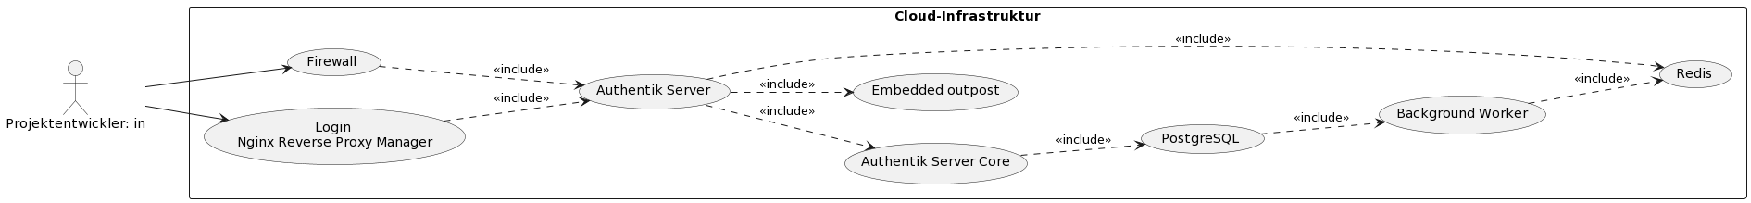
\includepdf[pages=-]{Use-Case-Diagram.pdf}
\rotatebox[origin=c]{90}{\includegraphicsKeepAspectRatio{Bilder/Use-Case-Diagram.pdf}{1}}
\caption{Use Case-Diagramm}
\end{figure}
\clearpage

\subsection{Sequenzdiagramm}
\label{app:Sequenzdiagramm}
% \includegraphicsKeepAspectRatio{Sequenzdiagramm.pdf}{1}

\subsection{Cloud-Infrastruktur}
\label{app:Cloud-Infrastruktur}
\includegraphicsKeepAspectRatio{Bilder/Infrastruktur1.pdf}{1}
\includegraphicsKeepAspectRatio{Bilder/Infrastruktur2.pdf}{1}
\clearpage

\subsection{Benutzerdokumentation}
\label{app:Benutzerdokumentation}
\clearpage


\end{document}
